\chapter{Probabilistic rules}
\label{chap:rules}

This chapter spells out the dialogue modelling approach developed in this thesis.  The previous chapter demonstrated how graphical models can help reduce the complexity of probability and utility models by exploiting independence properties between variables. We argued that factorised representations offered a number of theoretical and practical advantages for various learning and inference tasks. But despite these attractive properties, graphical models do also unfortunately suffer from scalability problems when faced with complex dialogue domains.  Conditional dependencies between variables can lead to an rapid increase in the number of distributions included in the model. Alas, only limited amounts of training data are available for most dialogue domains.  Estimating the model distributions in such setting is therefore a challenging task. 

To address this issue, we introduce in this chapter the notion of \textit{probabilistic rules}, which are structured mappings between conditions and  (parametrised) effects.  These rules function as \textit{high-level templates} for the construction of a dynamic decision network.  The key advantage of such structured modelling approach is the drastic reduction of the number of parameters compared to traditional representations.  We also argue that these expressive representations are particularly well suited to encode the probability and utility models used in dialogue management, where substantial amounts of expert knowledge can be leveraged to structure the relationships between variables. 

The chapter is divided in six sections:  Section \ref{sec:rmotivation} demonstrates in general terms how structural assumptions can be used to refine the representation of probabilistic models. Section \ref{sec:prules} show such structural assumptions can be practically encoded with probabilistic rules.  We formally define these rules in terms of conditions and effects and provide some concrete examples of rules for dialogue management.  Section \ref{sec:ruleinstantiation} connects these definitions to the graphical models described in the previous chapter by showing how probabilistic rules are practically instantiated into a graphical model.  Finally, Section \ref{sec:amodelling} addresses some advanced modelling issues and Section \ref{sec:relatedwork} relates the approach to previous work.


\section{Structural assumptions}
\label{sec:rmotivation}

The starting point of our approach is the observation that probability and utility models used in dialogue management often exhibits a fair amount of \textit{internal structure}.  
We have already discussed in the previous chapter one simple instance of this internal structure, based on factored representations. However, the internal structure of dialogue domains does not limit itself to these basic forms of conditional independence. 

%If two sets of random variables $\mathbf{X}$ and $\mathbf{Y}$ are conditionally independent given $\mathbf{Z}$, we can rewrite the probability distribution $P(\mathbf{X}, \mathbf{Y} \, | \, \mathbf{Z})$ as $P(\mathbf{X} \, | \, \mathbf{Z}) (\mathbf{Y} \, | \, \mathbf{Z}) $.  


\subsubsection*{Latent variables}
 
The number of parameters required to estimate the distributions of a graphical model can often be reduced by introducing \textit{latent variables} (i.e. unobserved or hidden variables) as intermediaries between the source and target variables. Indeed, many application domains are often best explained by the combination of a small number of distinct factors or influences, each encoded by a separate random variable and associated with a subset of input and output variables. Theses variables are usually never observed directly but contribute to structuring the model.\footnote{The use of layered computational models is one of the most active research topic in many areas of artificial intelligence and machine learning, and form in particular the foundations of deep learning approaches \citep{Bengio:2009}.} In the particular case of medical diagnosis, the relation between predisposing factors and observed symptoms are for instance preferably described by postulating an intermediary layer of variables -- possible diseases -- that mediate between the factors and the symptoms.  Figure \ref{fig:latentvariables} illustrates how a latent variables can be exploited to provide an additional layer of abstraction within a graphical model.

 \begin{figure}[h]
\centering
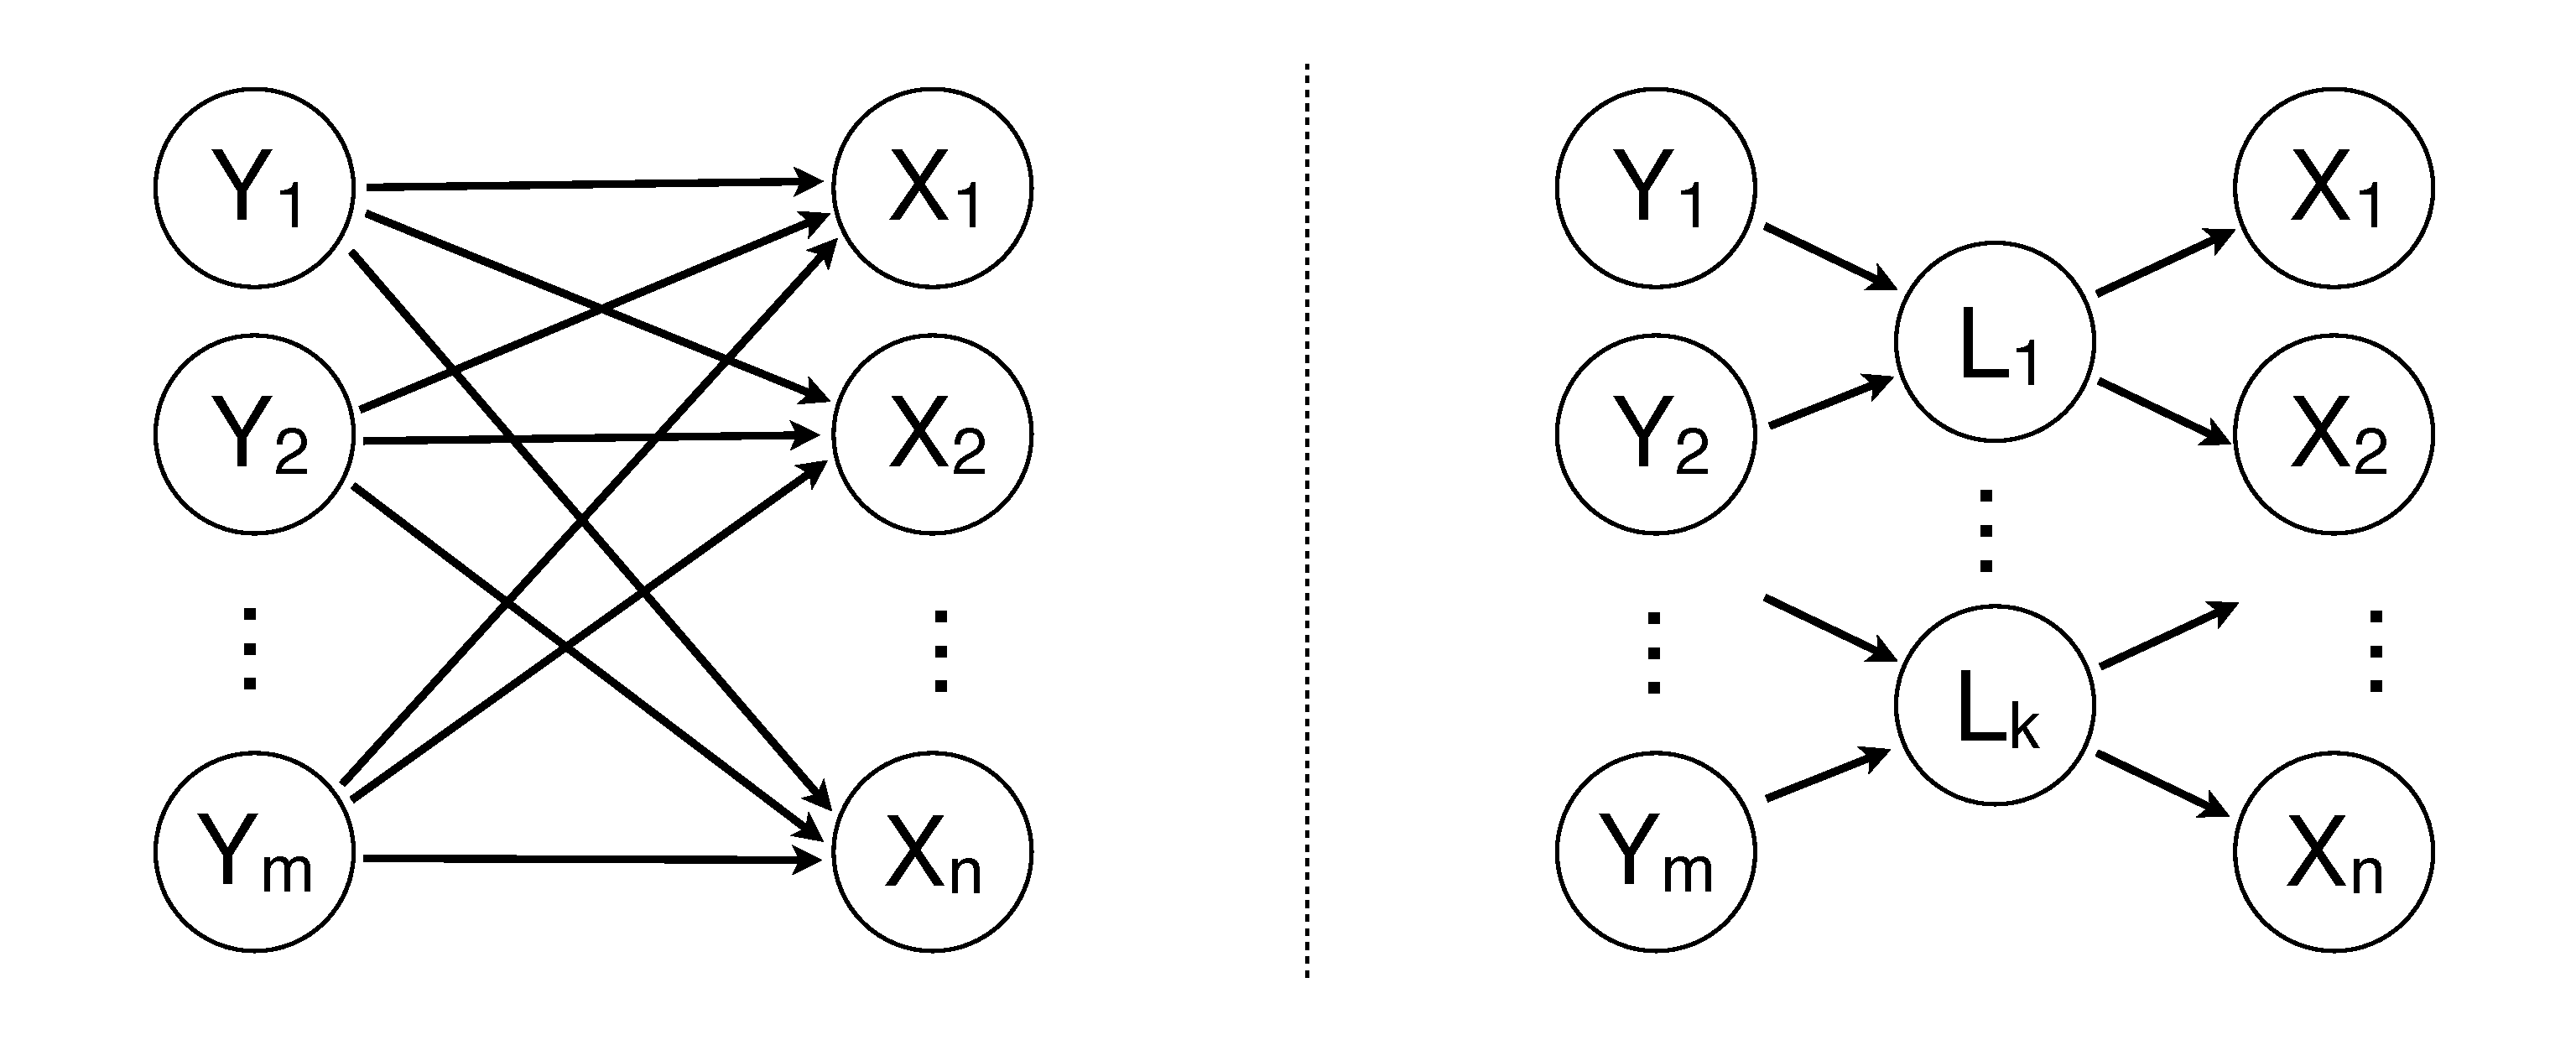
\includegraphics[scale=0.25]{imgs/latentvariables.pdf}
\caption{Comparison between a model that directly maps variables $\mathbf{Y}$ to $\mathbf{X}$ (left side) and one relying on latent variables $\mathbf{L}$ to serve as intermediaries (right side).}
\label{fig:latentvariables}
\end{figure}

Dialogue models can often benefit from introduction of such latent variables. The transition function can in particular be modelled in terms of a limited number of latent variables, each responsible for capturing specific aspects of the interaction dynamics. 

\subsubsection*{Partitioning}

A variable $X$ with $m$ parents $Y_1,...Y_m$ must specify a separate probability distribution for every possible assignment of values for the parent variables. In other words, the number of parameters required to specify the distribution $P(X \, | \, Y_1, Y_m)$ is exponential in the number of parents $m$. Fortunately, the values of these parents variables can be grouped into \textit{partitions} yielding similar outcomes for $X$. One can therefore directly define the conditional probability distributions on these groups than on the full enumeration of combined values for the parent variables. Partitioning is in essence an abstraction mechanism that allows us to reduce the model complexity and hence improve its ability to generalise to unseen examples. Utility distributions can also partition the values of their dependent variables in a similar way.  

As illustration, consider a minimalistic dialogue in a robot learning scenario where the robot can ask the user yes/no questions pertaining to the colour of one specific object (e.g. \utt{Is the object red?}). In this simple scenario, the state is represented with two variables: the user dialogue act $a_u = \{\mathit{yes,no}\}$ and a variable representing the object colour, $\mathit{colour} = \{\mathit{blue,green, ...}\}$ with $n$ possible colours.  The system actions take the form $a_m = \{ \mathit{VerifyColour(c)}: c \in \mathit{colour}\}$, where $VerifyColour(c)$ corresponds to asking the user whether the object is of colour $c$.  Since the object colour remains constant, the transition function for this domain is defined as $P(a_u'|a_m, \mathit{colour})$. The number of parameters required to specify the transition function is $n^2$ (since $a_m$ and $\mathit{colour}$ have $n$ possible values each). 

However, one can reasonably assume in this example that the particular colour mentioned in the question is irrelevant to predict the next user dialogue act $P(a_u'|a_m,\mathit{colour})$ as long as it matches (or fails to match) the actual colour of the object.  Based on this assumption, one can divide the space $Val(a_m) \times Val(\mathit{colour})$ into two distinct partitions: 
\begin{enumerate}
\item One partition in which the verification question corresponds to the actual colour of the object: $\exists c: colour\!=\!c \land a_m\!=\!\mathit{VerifyColour(c)}$.
\item One partition in which there is a mismatch between the colour mentioned in the question and the actual colour: $\exists c: colour\!=\!c \land a_m\!\neq\!\mathit{VerifyColour(c)}$.
\end{enumerate}

By abstracting over the specific colour mentioned in the question, partitioning allows us to drastically reduce the number of parameters required for the conditional probability distribution $P(a_u'|a_m,\mathit{colour})$ from a total of $n^2$ to only $2$. Figure \ref{fig:partitioning} illustrates this reduction. It is important to note that the action of grouping value assignments into partitions is a modelling choice, and can degrade the model accuracy if the partitions do not reflect actual concordances in the predicted outcomes -- for instance, the suggested partitions would be a poor modelling choice in case of a color-blind user unable to recognise certain colours. 

 \begin{figure}[h]
\centering
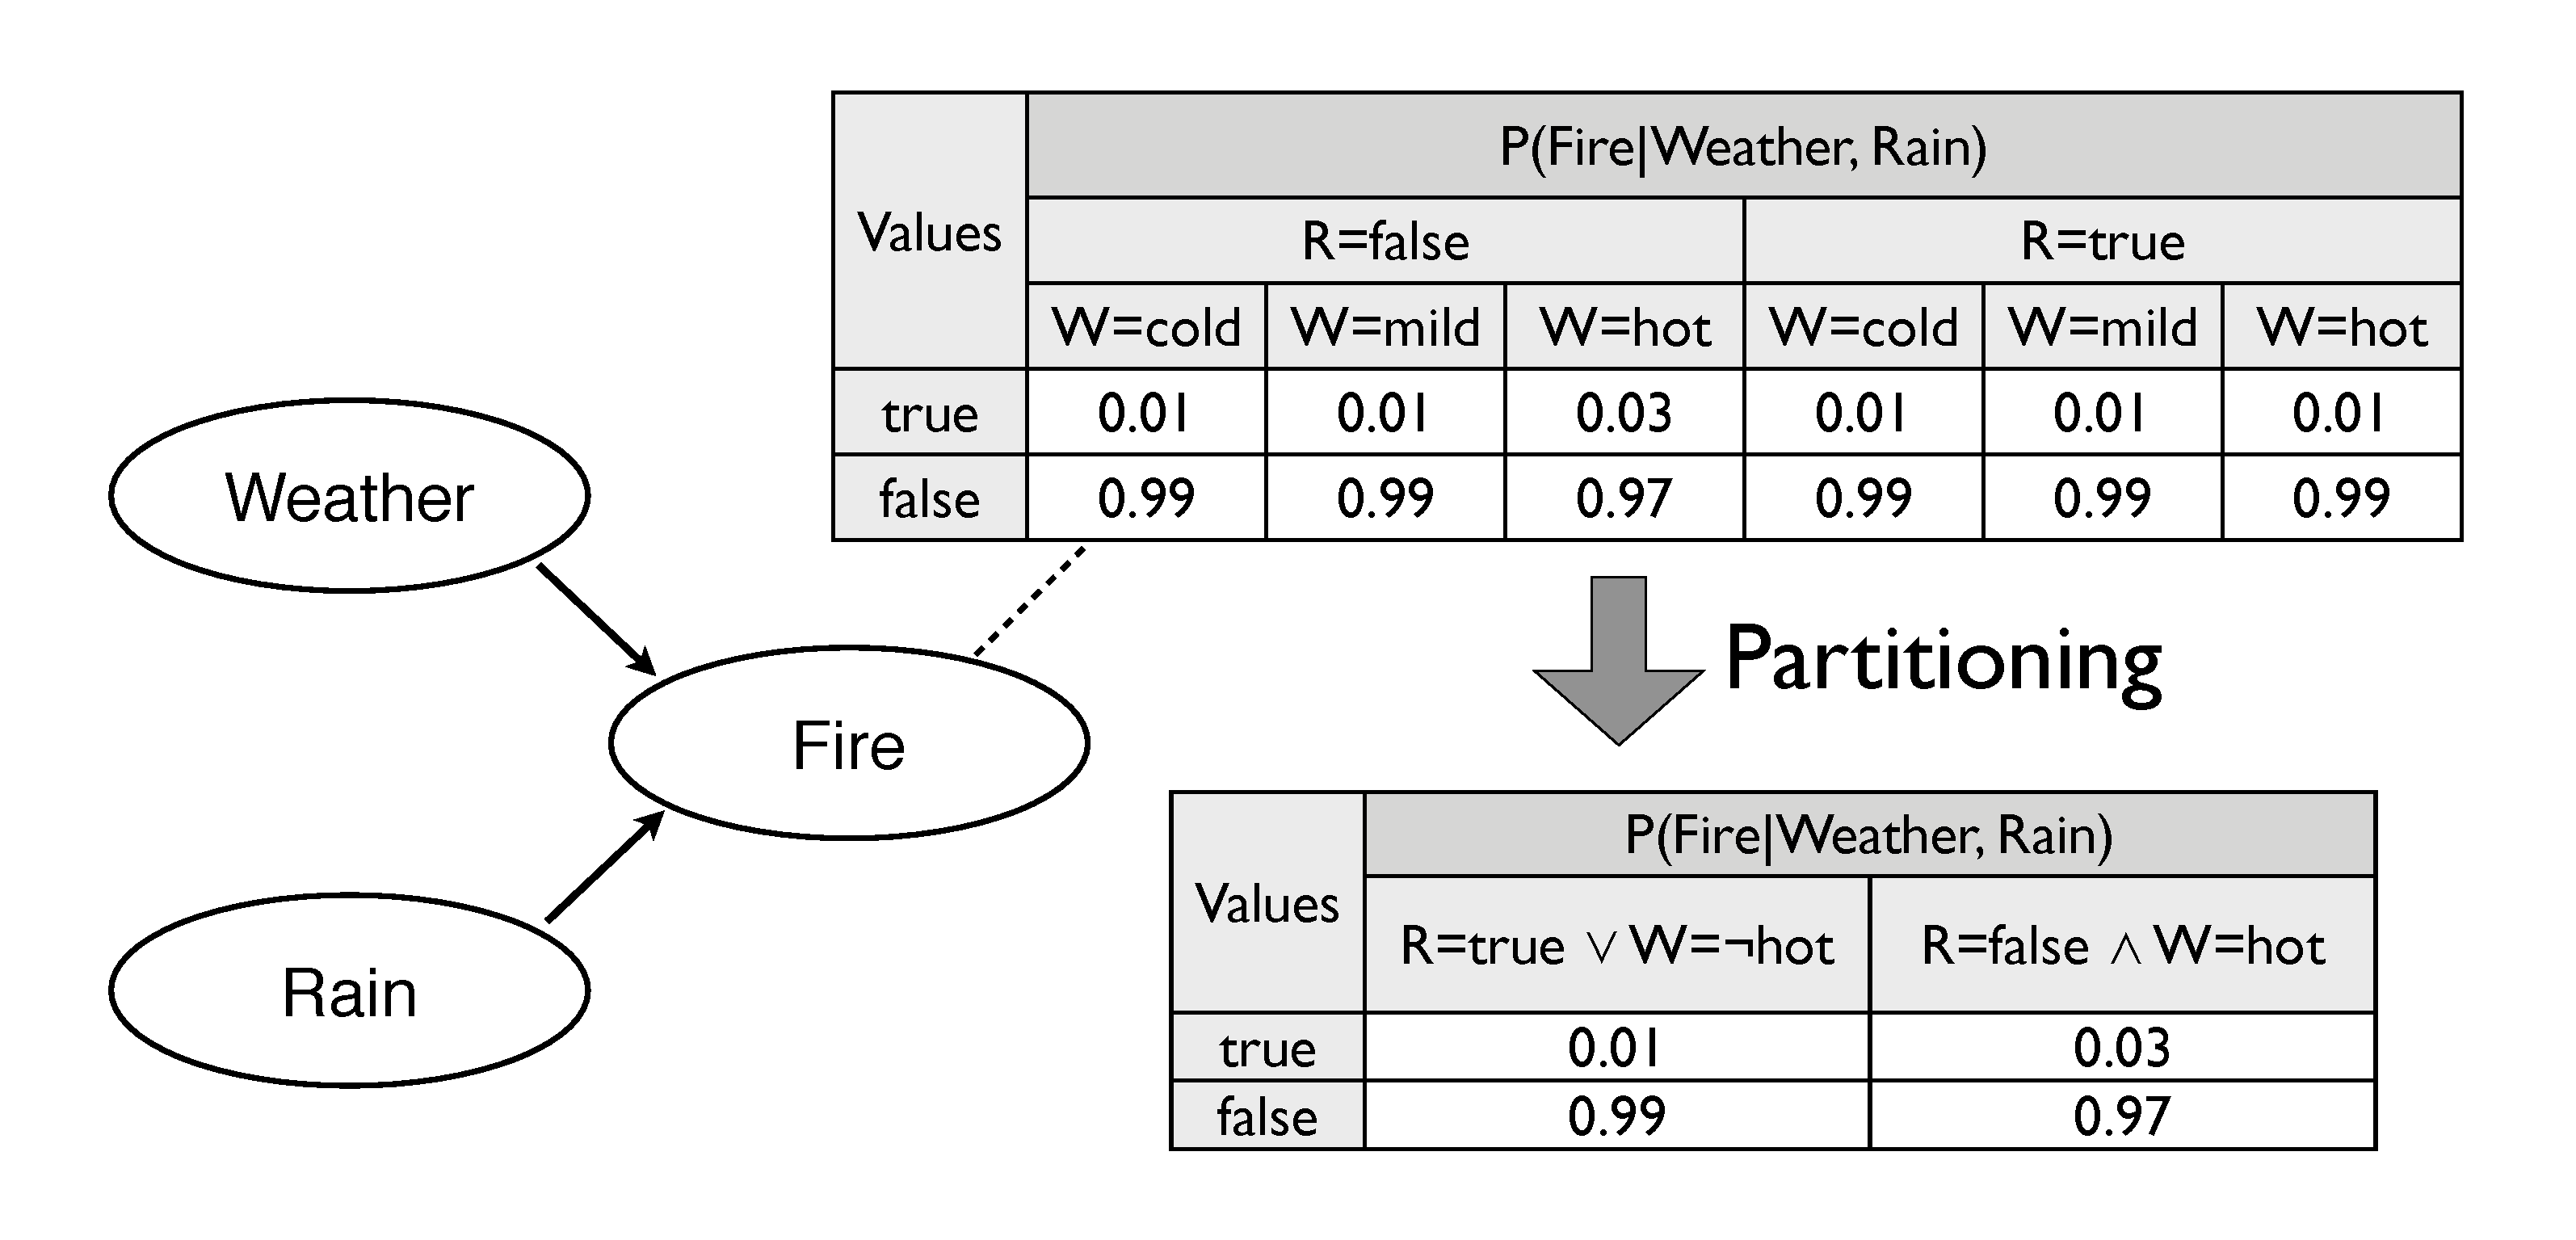
\includegraphics[scale=0.25]{imgs/partitioning.pdf}
\caption{Example of partitioning for the conditional probability distribution $P(a_u'|a_m,\mathit{colour})$.}
\label{fig:partitioning}
\end{figure}

Partitions must both exhaustive (each combination of values for the parent variables must belong to one partition) and mutually exclusive (a combination of values can only belong to one partition).  As we can observe from the example, partitions can often be concisely expressed via logical conditions on the variable values.  A given assignment of values will then be grouped in a partition if it satisfies the condition associated with it.

\subsubsection*{Relational structures}

Many dialogue domains cannot be easily described by a fixed set of random variables.  Situated domains such as human-robot interaction might for instance need to represent a varying number of perceived objects in the dialogue state.  These entities can be related with one another with multiple relations.  Examples of such relational structure of entities include:
\begin{itemize}
\item Collections of physical objects in a visual scene, each described by specific features (colour, shape) and relations with other objects (e.g. spatial relations),
\item Indoor environments topologically structured in rooms and spaces in which to navigate, 
\item Stacks of tasks to complete by the agent, each task being possibly connected to other tasks via precedence or inclusion relationships.
\end{itemize}

First-order logic provides an excellent basis for representing and manipulating such relational structures, as it offers a rich language for referring to objects connected with one another through functions and relations and describing their general properties in a concise way through the use of universal and existential quantifiers.\footnote{We shall not cover in this thesis the mathematical foundations of first-order logic, but the interested reader is invited to refer to e.g. \cite{gamut1991logic} for a formal overview of the logical concepts mentioned throughout this thesis.}. 

Graphical models can be extended to represent such relational domains by instantiating one random variable for every possible grounding of the functions and predicates for the domain.  For instance, a domain with two objects $o_1$ and $o_2$ and a relation $\mathit{leftOf}(x,y)$ will generate the four groundings $\mathit{leftOf}(o_1,o_2)$, $\mathit{leftOf}(o_2,o_1)$ $\mathit{leftOf}(o_1,o_1)$ and $\mathit{leftOf}(o_2,o_2)$. However, the definition of probability and utility distributions that can handle the relational semantics of such representation is however not straightforward.  One must indeed often define properties or constraints that are independent of the particular object being considered, such as $\forall x, \neg \mathit{leftOf}(x,x)$ and $\forall x, y, z, \mathit{leftOf}(x,y) \land \mathit{leftOf}(y,z) \Rightarrow \mathit{leftOf}(x,z)$. Classical probabilistic models offer unfortunately no direct support for quantifiers, as their expressive power is intrinsically limited to propositional logic. 

The unification of first-order logic and probability theory has spanned a new research area called \textit{statistical relational learning} \citep{getoor:srlbook07}. Many of the methods developed in this field operate by defining a logic-based description language on top of classical probabilistic models that allow for some form of quantification. This description language is then used as a template to generate a classical probabilistic model given a set of constants. Similarly to the partitions described in the previous section, the introduction of quantifiers provide another abstraction mechanism to reduce the complexity of a given probabilistic models by describing constraints or relations that hold for all possible groundings of a given formula and might therefore apply to a large set of random variables. 

\section{Definitions}

We outline below a generic description framework for expressing this internal structure, based on the concept of \textit{probabilistic rules}.  The rules express the distribution of a dialogue model in terms of structured mappings between input and output variables.  At runtime, the rules are then combined to perform inference on the dialogue state, i.e. to compute the distribution of the output variables given the input variables. As we shall see, this is done by instantiating the rules and their associated variables to construct an equivalent Bayesian Network used for inference.  The probabilistic rules thus function as high-level \textit{templates} for a classical probabilistic model.  The major benefit of this approach is that the rule structure is described in exponentially fewer parameters than its plain counterpart, and is thus much easier to learn and to generalise to unseen data.  


\label{sec:prules}

\note{if then else automatically ensures that the partitions are mutually exclusive}

\subsection{Conditions}

\note{not string matching stuff}

\subsection{Effects}

\note{only the basics -- not addition, removal effects etc.}

\subsection{Parameters}

\subsection{Rule types}

\subsection{Examples}

\section{Rule instantiation}
\label{sec:ruleinstantiation}

\subsection{Dialogue state}

\note{Our approach is based on information state}

\note{like probabilistic pICI average models}

\note{fully defined relation -- no need for cases!}
\note{relation will then be extended to deal with more sophisticated effects (adds, etc.)}


\begin{align}
& P(X' = x' \, | \, R_1 = r_1,... R_n = r_n, X = x) = \frac{\mathbf{1}_{M} (r_1,...r_n, x, x')} { \text{card}(M(r_1,...r_n,x))}
\end{align}

\note{probabilistic ICI?  property of being decomposable, symmetric}

\subsection{Instantiation algorithm}

\subsection{Pruning mechanisms}

\section{Advanced modelling}
\label{sec:amodelling}

\subsection{Strings, numbers and collections}

\subsection{Quantifiers}

\section{Related work}
\label{sec:relatedwork}

\note{Heriberto's relational state: \cite{pub5502} an hierarchical aproach \citep{Heriberto2011}}. 

\section{Conclusion}

